\documentclass[journal,12pt,onecolumn]{IEEEtran}
\renewcommand\IEEEkeywordsname{Keywords}
%
\usepackage[utf8]{inputenc}
\usepackage[T1]{fontenc}
\usepackage{textcomp}
\usepackage{gensymb}
\usepackage{blindtext}
\usepackage{enumitem}
\setlist{parsep=0pt,listparindent=\parindent}
\usepackage{amsmath}
\usepackage{float}
\usepackage{caption}
\usepackage{placeins}
\usepackage{lipsum}  
\usepackage[final]{graphicx}
\usepackage{caption}
\usepackage{subcaption}
\extrafloats{100}
\usepackage{cite}
\usepackage{listings}
\usepackage{color}
\usepackage{listings}
\usepackage{amsfonts}
\usepackage{array,multirow}
\usepackage{tabularx}
\usepackage{pdfpages}


\newfloat{lstfloat}{htbp}{lop}
\floatname{lstfloat}{Listing}
 
\definecolor{codegreen}{rgb}{0,0.6,0}
\definecolor{codegray}{rgb}{0.5,0.5,0.5}
\definecolor{codepurple}{rgb}{0.58,0,0.82}
\definecolor{backcolour}{rgb}{0.95,0.95,0.92}
\lstdefinestyle{mystyle}{
   % backgroundcolor=\color{backcolour},   
    commentstyle=\color{codegreen},
   % keywordstyle=\color{Black},
    numberstyle=\tiny\color{codegray},
    stringstyle=\color{codepurple},
    basicstyle=\footnotesize,
    breakatwhitespace=false,         
    breaklines=true,     
    postbreak=\mbox{\textcolor{red}{$\hookrightarrow$}\space}            ,
    captionpos=b,                    
    keepspaces=true,                 
    numbers=none,                    
    numbersep=0pt,                  
    showspaces=false,                
    showstringspaces=false,
    showtabs=false,                  
    tabsize=2
}
\lstset{emph={%  
    End, If, While, then, Else, break, do, find_virtual_runway, model_wind, final_point , reverse, along_heading_at_distance, find_no_wind_air_trajectory,difference, null, return %
    },emphstyle={\bfseries}%
}
\renewcommand{\lstlistingname}{Pseudocode} 
\lstset{style=mystyle}

\renewcommand{\floatpagefraction}{.8}%
 
\newcommand*{\vect}[1]{\overrightarrow{#1}} 
 
%%%%%%%%%%%%%%%%%%%%%%%%%%%%%%%%%%%%%%%%%%%%%%%%%%%%%%%%%%%%%%%%%%
\begin{document}

\title{A Study of Factors Affecting Heart Disease Mortality Rate in the United States}

\author{
\IEEEauthorblockN{
Ashraful Islam,
Nicholas Luczak, 
Saswata Paul, and
Yiyun Su
}\\
\IEEEauthorblockA{
Rensselaer Polytechnic Institute, Troy, New York, 12180\\
\{islama6, luczan, pauls4, suy4\}@rpi.edu
}
}

\maketitle

\begin{abstract}
Coronary heart disease has become one of the major complications that ail the American population. 
So, in this paper, we investigate the factors that may be responsible for coronary heart disease in the United States.
We perform two types of analysis - an analysis of coronary heart disease and median household income for New York State and an analysis of coronary heart disease and social determinants for the entire United States.
We obtain public domain data from www.cdc.gov and www.data.gov to perform our analysis.
Our preliminary analysis shows interesting patterns between coronary heart disease mortality and social factors.
We then train a machine learning model to see if it is possible to correctly predict coronary heart disease from the various factors. 
 \end{abstract}
\section{Choosing the Investigation and Identifying a Pre-Existing Source of Data}
\subsection{The Goal and Reasons behind Choice of Datasets, How They Were Found and Managed}
We wanted to find datasets that were collected between the same time period, so that the analysis would be accurate.
We searched for suitable datasets in data.gov and cdc.gov and came across the heart disease mortality dataset. 
We realized that it was a rich dataset since it contained detailed information about heart disease mortality rate by county for the entire United States.
Then we decided that we wanted to do an analysis of how heart disease mortality is related to different social determinants.
We found two more rich datasets, the first of which contained information about median income for the state of New York and the other contained information about social determinants for the entire United States.

We stored and managed the datasets in a Github repository that we had created for the project.
All other materials related to the project were also stored there.   

\begin{figure}[H]
\caption{Project workflow}
\centering
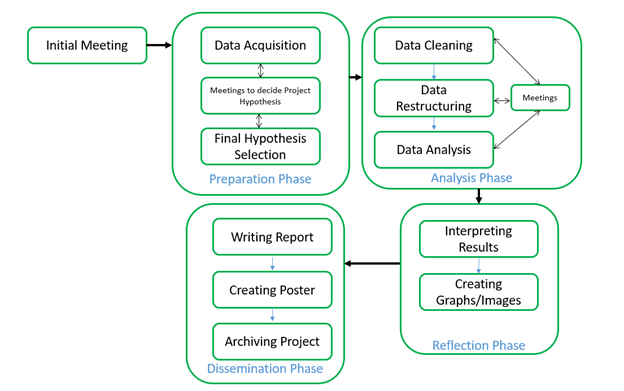
\includegraphics[width=0.75\textwidth]{figures/workflow.PNG}
\end{figure}
	
Given below is a description of the various stages of our project work:
\begin{itemize}
\item \textbf{Preparation Phase:}
In this phase, we downloaded several datasets from data.gov and cdc.gov. We looked at different types of datasets before deciding what the hypothesis of our project would be. We finalized a hypothesis after rejecting several options.
\item \textbf{Analysis Phase:}
In this phase, we cleaned the data and preprocessed it so that we could analyze it. For the median income dataset, there were multiple values for each county in the dataset, so we took an average of all the values for each county. We also had to make sure that the county names in the median income dataset were written exactly the same as in the heart disease dataset so that we could easily compare them using Excel. Moreover, there were erroneous and missing values that needed to be filtered.
\item \textbf{Reflection Phase:}
In this phase, we generated visual representations to support our hypothesis. We generated graphs, heatmaps and geo-distribution maps that corroborate our findings from the data. This helped us articulate and express our results in a way that is easily understandable by others.
\item \textbf{Dissemination Phase:}
In this phase, we aim to create the final report and the poster. We will also properly archive our project in the Github repository of the course. Data preservation will be handled by data.gov as the data was collected directly from that website. We will be providing copies of the datasets along with metadata and provenance information, but the most well documented source will still be the data.gov websites from where the data was originally collected.
\end{itemize}

\subsection{Data Formats and Metadata Standards}
A detailed description about the datasets is presented below.
\begin{enumerate}
\item \textbf{NYSERDA Low- to Moderate-Income New York State Census Population Analysis Dataset: Average for 2013-2015}
\begin{itemize}
\item	Collected from – catalog.data.gov
\item	Type of file – comma separated values
\item	Publisher - data.ny.gov
\item	Maintainer – NY Open data
\item	Maintainer email - openny@nyserda.ny.gov
\item	Unique Identifier - https://data.ny.gov/api/views/bui8-bb6g
\item	Metadata updated date – Nov 21, 2019
\item	Metadata created date – March 28, 2018
\end{itemize}

\begin{figure}[H]
\caption{A snippet of the NYSERDA Low- to Moderate-Income New York State Census Population Analysis Dataset.}
\centering
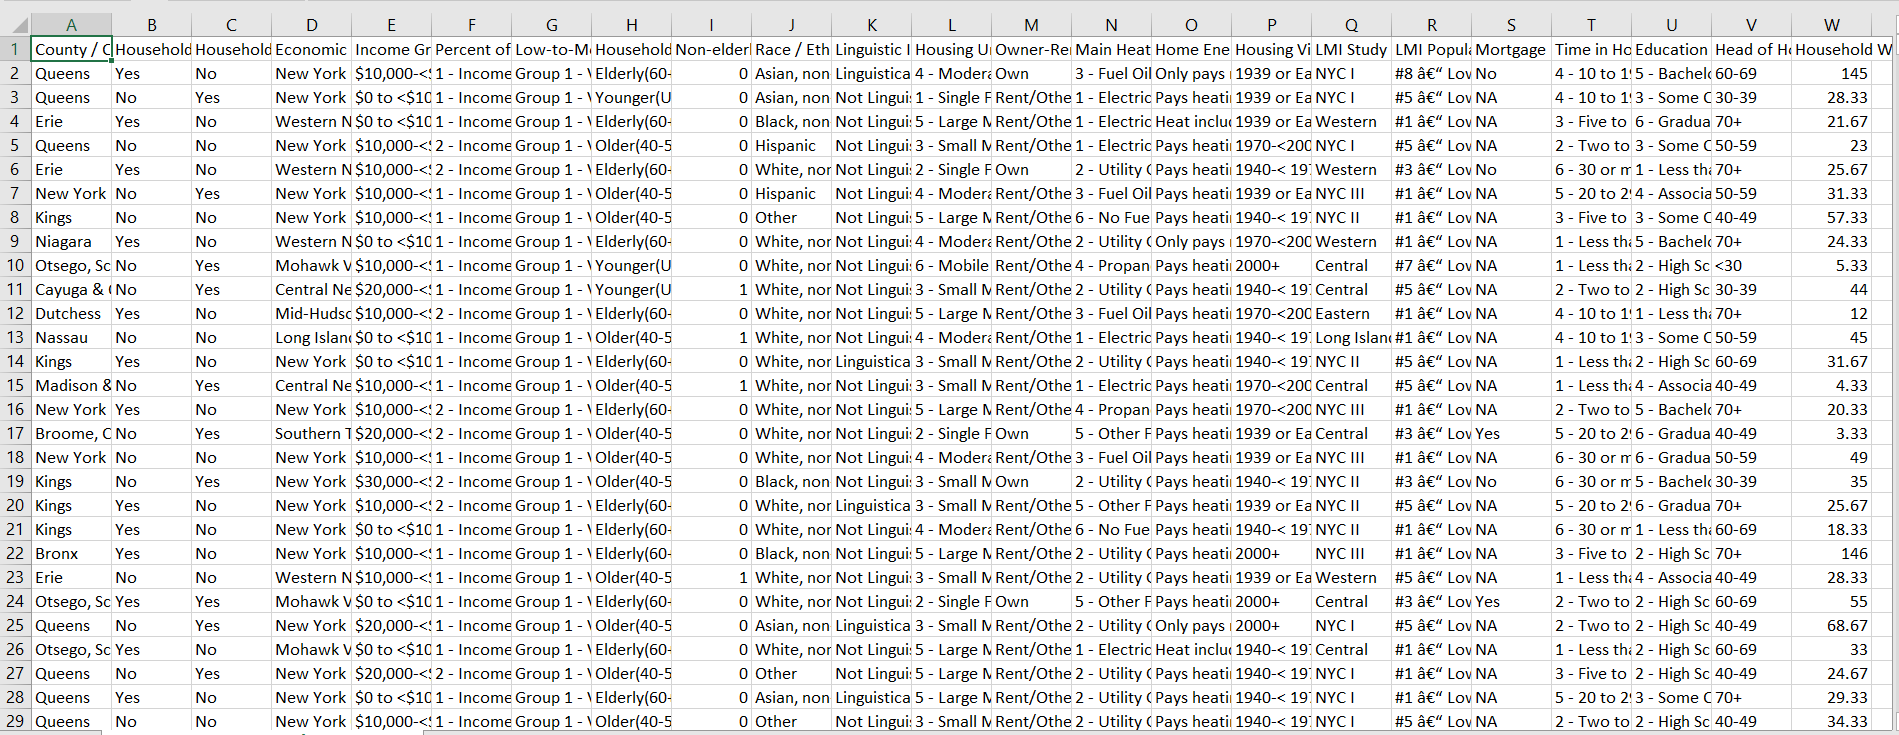
\includegraphics[width=\textwidth]{figures/data_mi.PNG}
\end{figure}

\item \textbf{Heart Disease Mortality Data Among US Adults (35+) by State/Territory and County}
\begin{itemize}
\item	Collected from – catalog.data.gov
\item	Type of file – comma separated values
\item	Publisher - Centers for Disease Control and Prevention
\item	Maintainer – DHDSP Requests
\item	Maintainer email - dhdsprequests@cdc.gov
\item	Unique Identifier - https://data.cdc.gov/api/views/i2vk-mgdh
\item	Metadata updated date – June 11, 2019
\item	Metadata created date – September 2, 2019
\end{itemize}

\begin{figure}[H]
\caption{A snippet of the Heart Disease Mortality Data Among US Adults Dataset.}
\centering
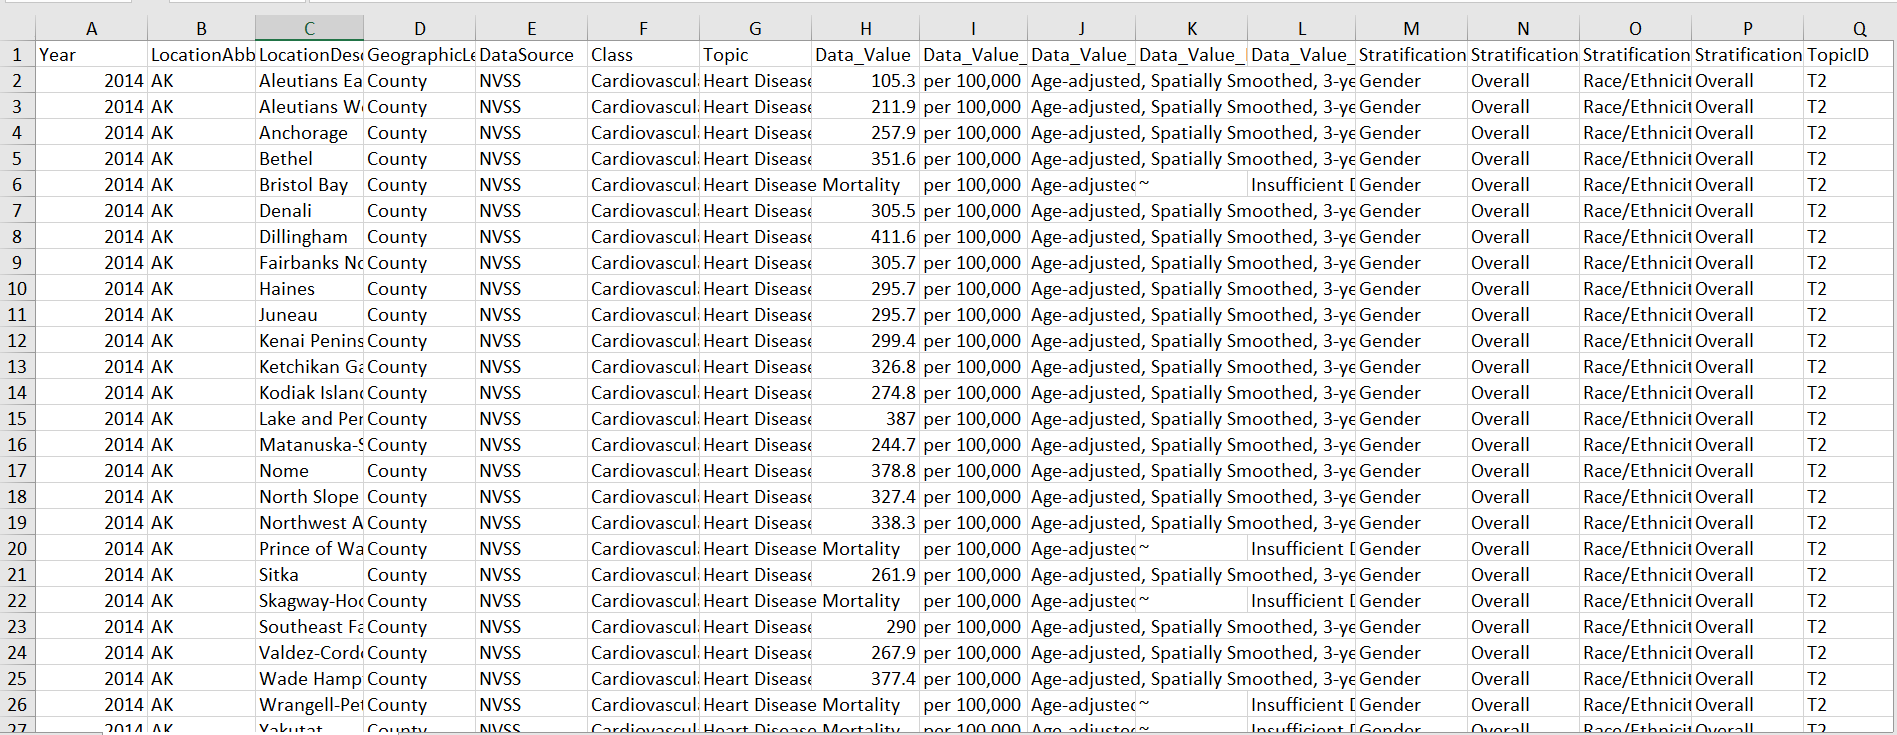
\includegraphics[width=\textwidth]{figures/data_hd.PNG}
\end{figure}


\item \textbf{Social Vulnerability Index 2012 - 2014}
\begin{itemize}
\item	Collected from – svi.cdc.gov
\item	Type of file – comma separated values
\item	Publisher - cdc.gov
\item	Maintainer – Centers for Disease Control and Prevention
\item	Maintainer email - dhdsprequests@cdc.gov
\end{itemize}

\begin{figure}[H]
\caption{A snippet of the Social Vulnerability Index Dataset.}
\centering
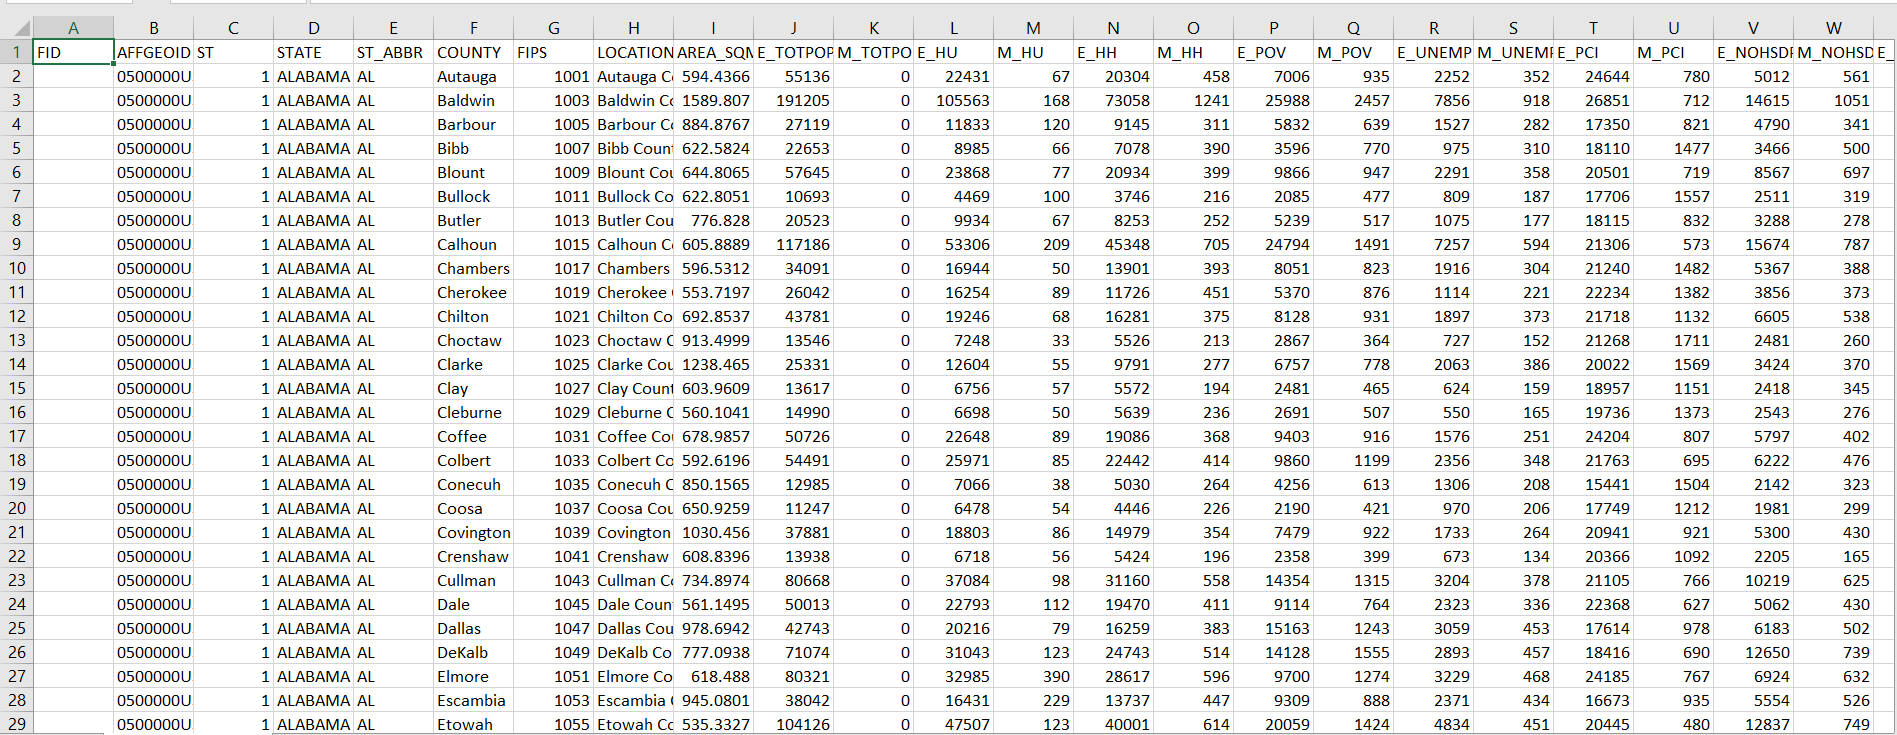
\includegraphics[width=\textwidth]{figures/data_svi.PNG}
\end{figure}


\end{enumerate}

The datasets that we used for this project were collected from data.gov and cdc.gov.
They were stored in an organized manner in csv formats, which made them easy to use without much pre-processing.
They were well documented, which made it easy to work with them without much confusion.

\section{Data Analysis}

\subsection{The Questions/Hypotheses we Sought to Answer from the Data}
Since the datasets we chose had rich information about heart disease mortality rate, median income for New York State, and social determinants, we decided to answer the two following questions:
\begin{enumerate}
\item \emph{How is heart disease mortality rate connected to the median income in New York State?}
\item \emph{How is heart disease mortality rate connected to social vulnerability in the United States?}
\item \emph{How is heart disease mortality rate connected to ethnicity?}
\end{enumerate} 

We first decided to check using basic exploratory data analysis if there was actually any relationship between heart disease mortality rate and the other factors as explained above.  
For that we planed to use MS Excel.
After a pattern was found, we decided to clean the data and do some pre-processing so that the relationships could be studied in detail.
After we were certain that there were some clear relationships between the factors, we decided to train a machine learning model to try and see if we could predict heart disease mortality from social determinants.

\subsection{Description of Tools and Methods used for the Analysis}
\begin{itemize}
\item Python was used for cleaning and pre-processing the data for analysis of the first hypothesis.
We first cleaned the data by filtering all missing and erroneous fields, then we pre-processed it by taking only the counties that were common in both datasets.
We also needed to manually split some county names which had been grouped together median income dataset during data cleaning.
Two different pieces of code were written - \emph{data\_clean.py} for cleaning the data and \emph{data\_fix.py} for pre-processing the data
The codes are given in Appendix I.

\item For creating a machine learning model, we used the scikit-learn tool and the Pandas tool to read the data and create data frames in Python.
The entire code for the machine learning part is given in the Appendix II.

\item For the visualizations of the analysis of the relationship between heart disease mortality rate and median income, Microsoft Excel was used.

\item To draw the choloropeth maps for the social vulbnerability index distribution, we used a software called arcGis.
\end{itemize}


\subsection{Steps Taken to Perform the Analysis}

\subsubsection{For the Analysis of Relationship Between Heart Disease Mortality Rate and Median Income for New York State}
\begin{enumerate}
\item First, we had to clean the data and remove rows with missing fields.
\item In the NYSERDA dataset, the data was presented in a way in which multiple counties were bundled together.
So, we had to write a Python script to manually separate the counties.
\item Once the  NYSERDA dataset was cleaned, we had to save it as a new file.
\item Then we had to extract data for NY state counties which were common in both the NYSERDA and Heart Disease Mortality datasets.
This was done with the help of a Python script.
\item For the analysis, we put the Heart Disease Mortality rate and Median income for each county as columns into a csv file.
Then we used MS Excel to analyze the data.
\end{enumerate}
\subsubsection{For the Analysis of Relationship Between Heart Disease Mortality Rate and Social Determinants for the entire United States}
\begin{enumerate}
\item First we downloaded the shape file of the data from the data download page of CDC.
\item Next, we used arcGis, a proprietary mappoing application to create the county map for the entire United States.
\item Then we used the different scores in the social vulnerability index to divide them into quartiles.
\item The on the map, we plotted the value for each county, with the four scores represented by 4 varying degrees of colors.
\end{enumerate}

\subsubsection{For the Creation of a Machine Learning Model and Testing it on the Data}
\begin{enumerate}
\item First, we had to clean the data and remove rows with missing fields.
\item From the Social Vulnerability Index data, the following fields were selected for analysis: 
\begin{itemize}
\item EP\_POV (person below poverty estimate),
\item EP\_UNEMP (civilian unemployed),
\item EP\_PCI (per capita income),
\item EP\_NOHSDP (person with no high school diploma),
\item EP\_AGE65 (person age 65+),
\item EP\_AGE17 (17+),
\item EP\_SNGPNT (single parent household with one children),
\item EP\_MINRTY (minority estimate except white, non-Hispanic),
\item EP\_LIMENG (person who speaks English less than well),
\item EP\_NOVEH (household with no vehicle),
\item EP\_GROUPQ (person in group quarters),
\item E\_TOTPOP (total population).
\end{itemize}
\item Python Scikit Learn was used to see the corelation between the different metrics.
\item The data was pre-processed to convert heart rate disease values to categorical values.
\item Python Scikit Learn was used to train SVM and KNN and analyze their accuracy (Details given in Appendix II).  
\end{enumerate}

\subsubsection{For the analysis of heart disease mortality rate and ethnicity}
For this analysis, we simply cleaned the data by removing rows with missing values and used Microsoft Excel to create a chart of how heart disease rate varies with ethnicity.


\section{Presentation/Visualization of the Results}
\subsection{Results of the Analysis}
\subsubsection{Relationship Between Heart Disease Rate and Median Income for New York State}
We used MS Excel to perform this analysis.
First we created a chart that compared the heart disease mortality rate to the median income for each state.
Since the heart disease mortality rate was too small compared to median income for the them to be clearly accommodated in a single column chart, we convert it from per 100000 to per 10000000.
Then we plotted the average line for both median income and heart disease rate.
We also created two choropleth maps of heart disease mortality rate and median income using MS Excel to see how they were related.

\begin{figure}[H]
\centering
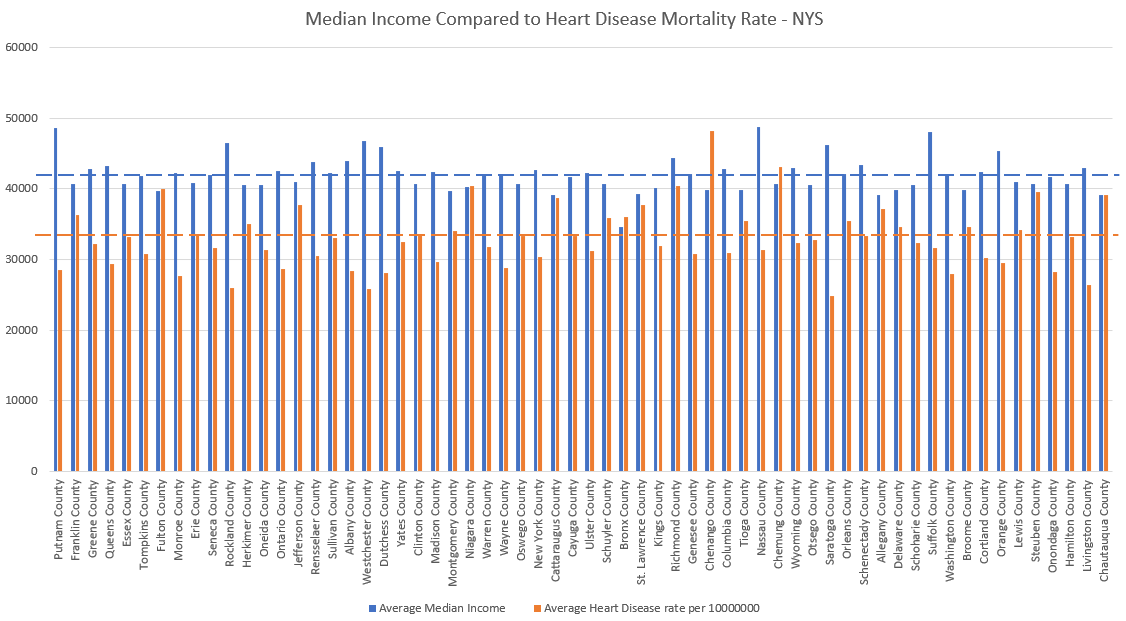
\includegraphics[width=\textwidth]{figures/column.PNG}
\caption{Heart disease mortality rate vs median income (NYS).}
\label{fig:col1}
\end{figure}


\begin{figure}[H]
  \centering
  \begin{subfigure}{.5\textwidth}
  \centering
  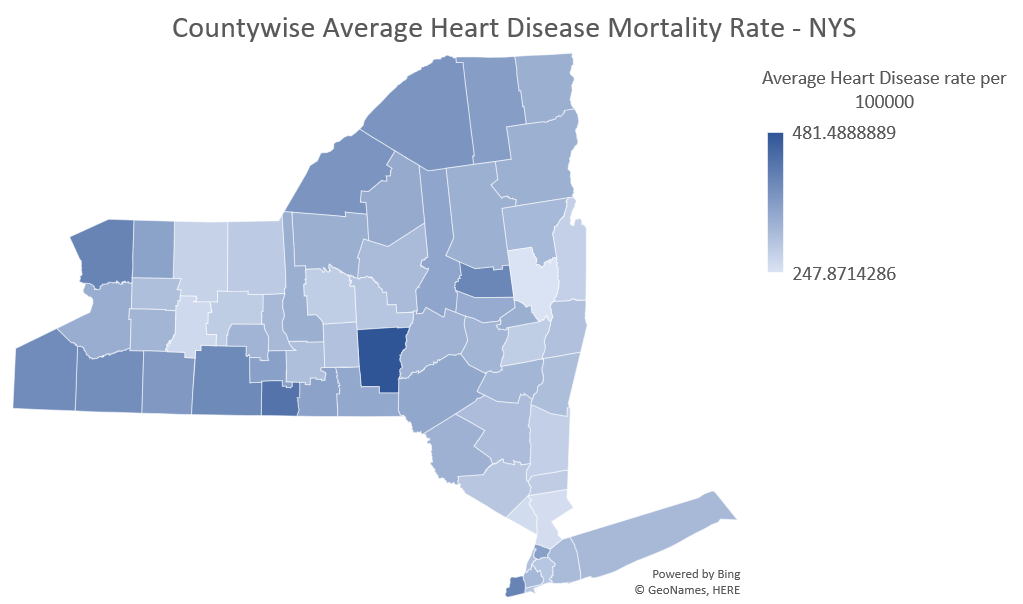
\includegraphics[width=\linewidth]{figures/map_heart.PNG}
  \caption{Heart disease mortality rate}
  \label{fig:hdmap}
\end{subfigure}%
\begin{subfigure}{.48\textwidth}
  \centering
  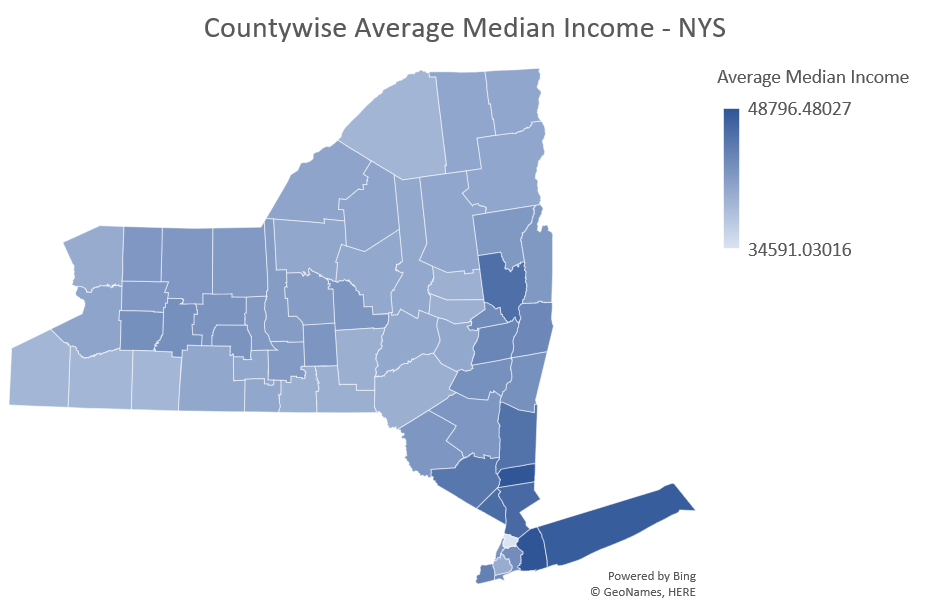
\includegraphics[width=\linewidth]{figures/map_income.PNG}
  \caption{Median income}
  \label{fig:hdheatmap}
\end{subfigure}
\caption{Median income vs heart disease mortality rate for New York}
\label{}
\end{figure}



\textbf{Results:}
From Fig. \ref{fig:col1}, it is clear that in in most counties where median income is below the average, heart disease rate is above average and vice versa.
This is corroborated by Fig. \ref{fig:hdmap} and Fig. \ref{fig:mimap} which show that in counties where median income is low, heart disease rate is high and vice versa.
Therefore we can conclude that heart disease mortality rate is usually inversely related to median income.   
\newpage
\subsubsection{Relationship Between Heart Disease Rate and Social Vulnerability}
\begin{center}
\centering
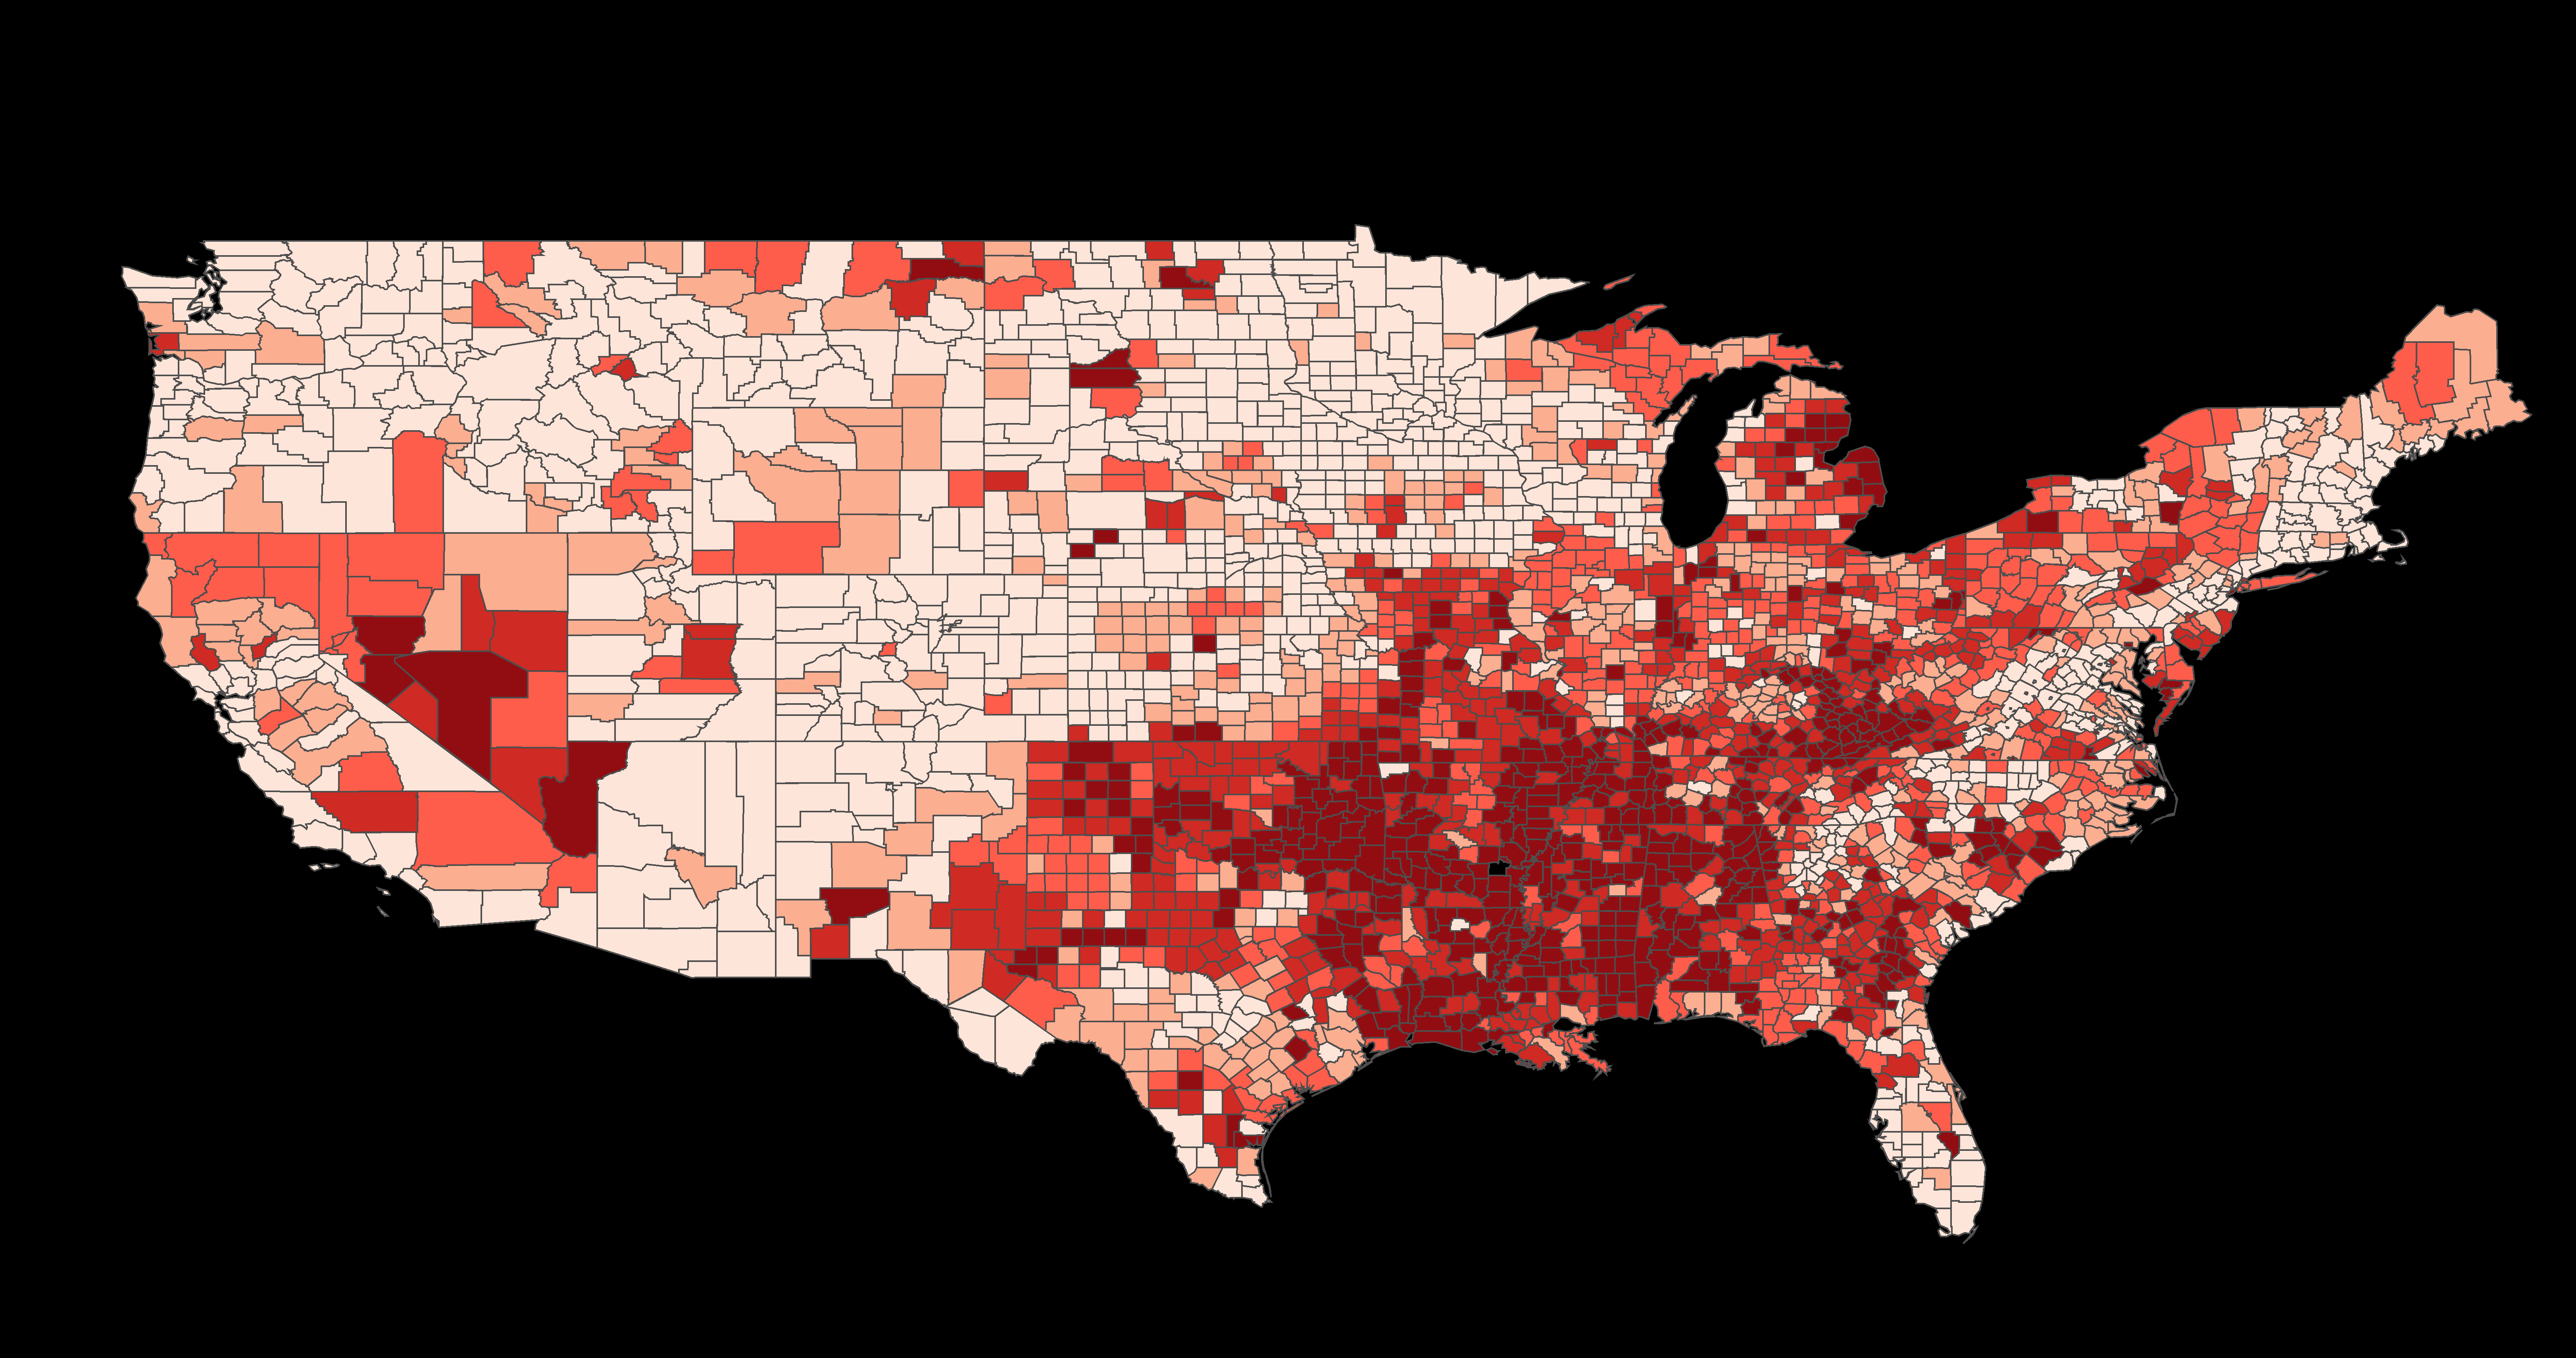
\includegraphics[width=0.8\textwidth]{figures/chloro_heart.PNG}
\captionof{figure}{Chloropeth map of heart disease mortality rate}
\label{fig:chloroheart}
\end{center}

\begin{center}
\centering
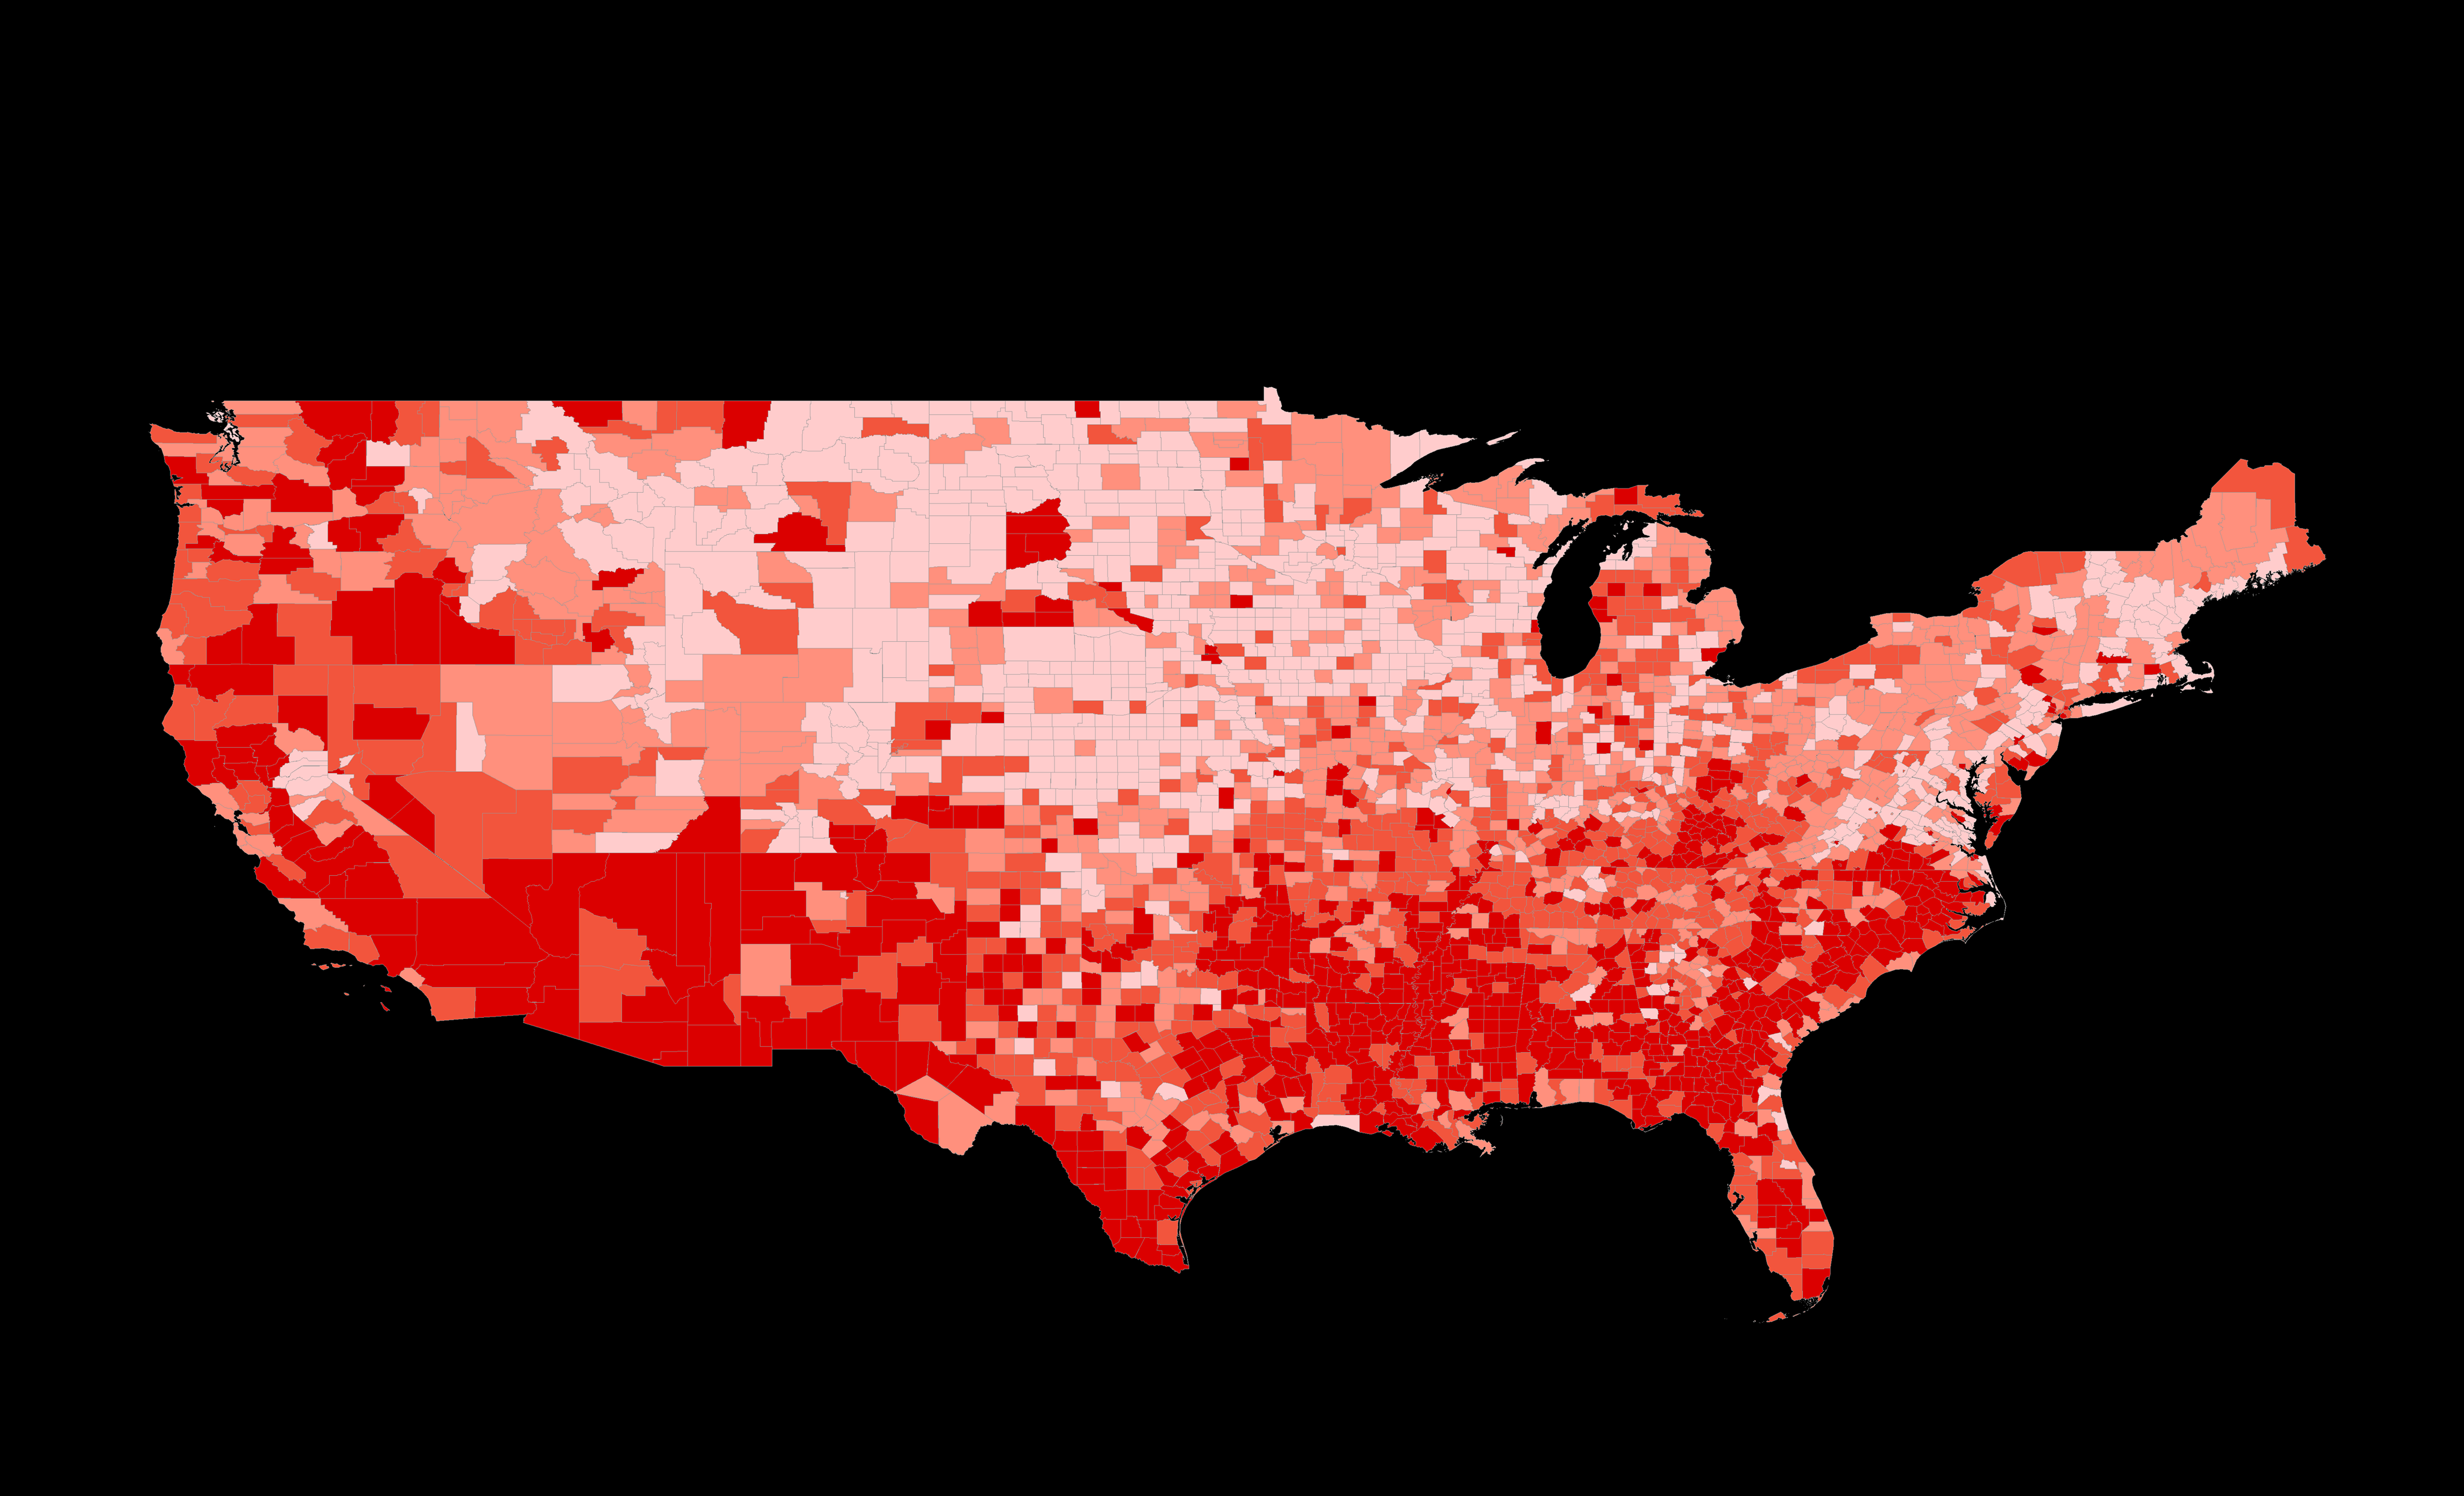
\includegraphics[width=0.8\textwidth]{figures/chloro_svi.PNG}
\captionof{figure}{Chloropeth map of overall social vulnerability index (2012-2014)}
\label{fig:chlorosvi}
\end{center}

It uses these 15 US census variables to determine the Social vulnerability of each county. 
We believe that these indicators of social vulnerability also serve as strong indicators of social determinants. 
Our hypothesis is that the higher the overall vulnerability of a community the less likely they are to live a healthy lifestyle; therefore, their likelihood of coronary-related mortalities sees an increase as a result. 

\begin{center}
\centering
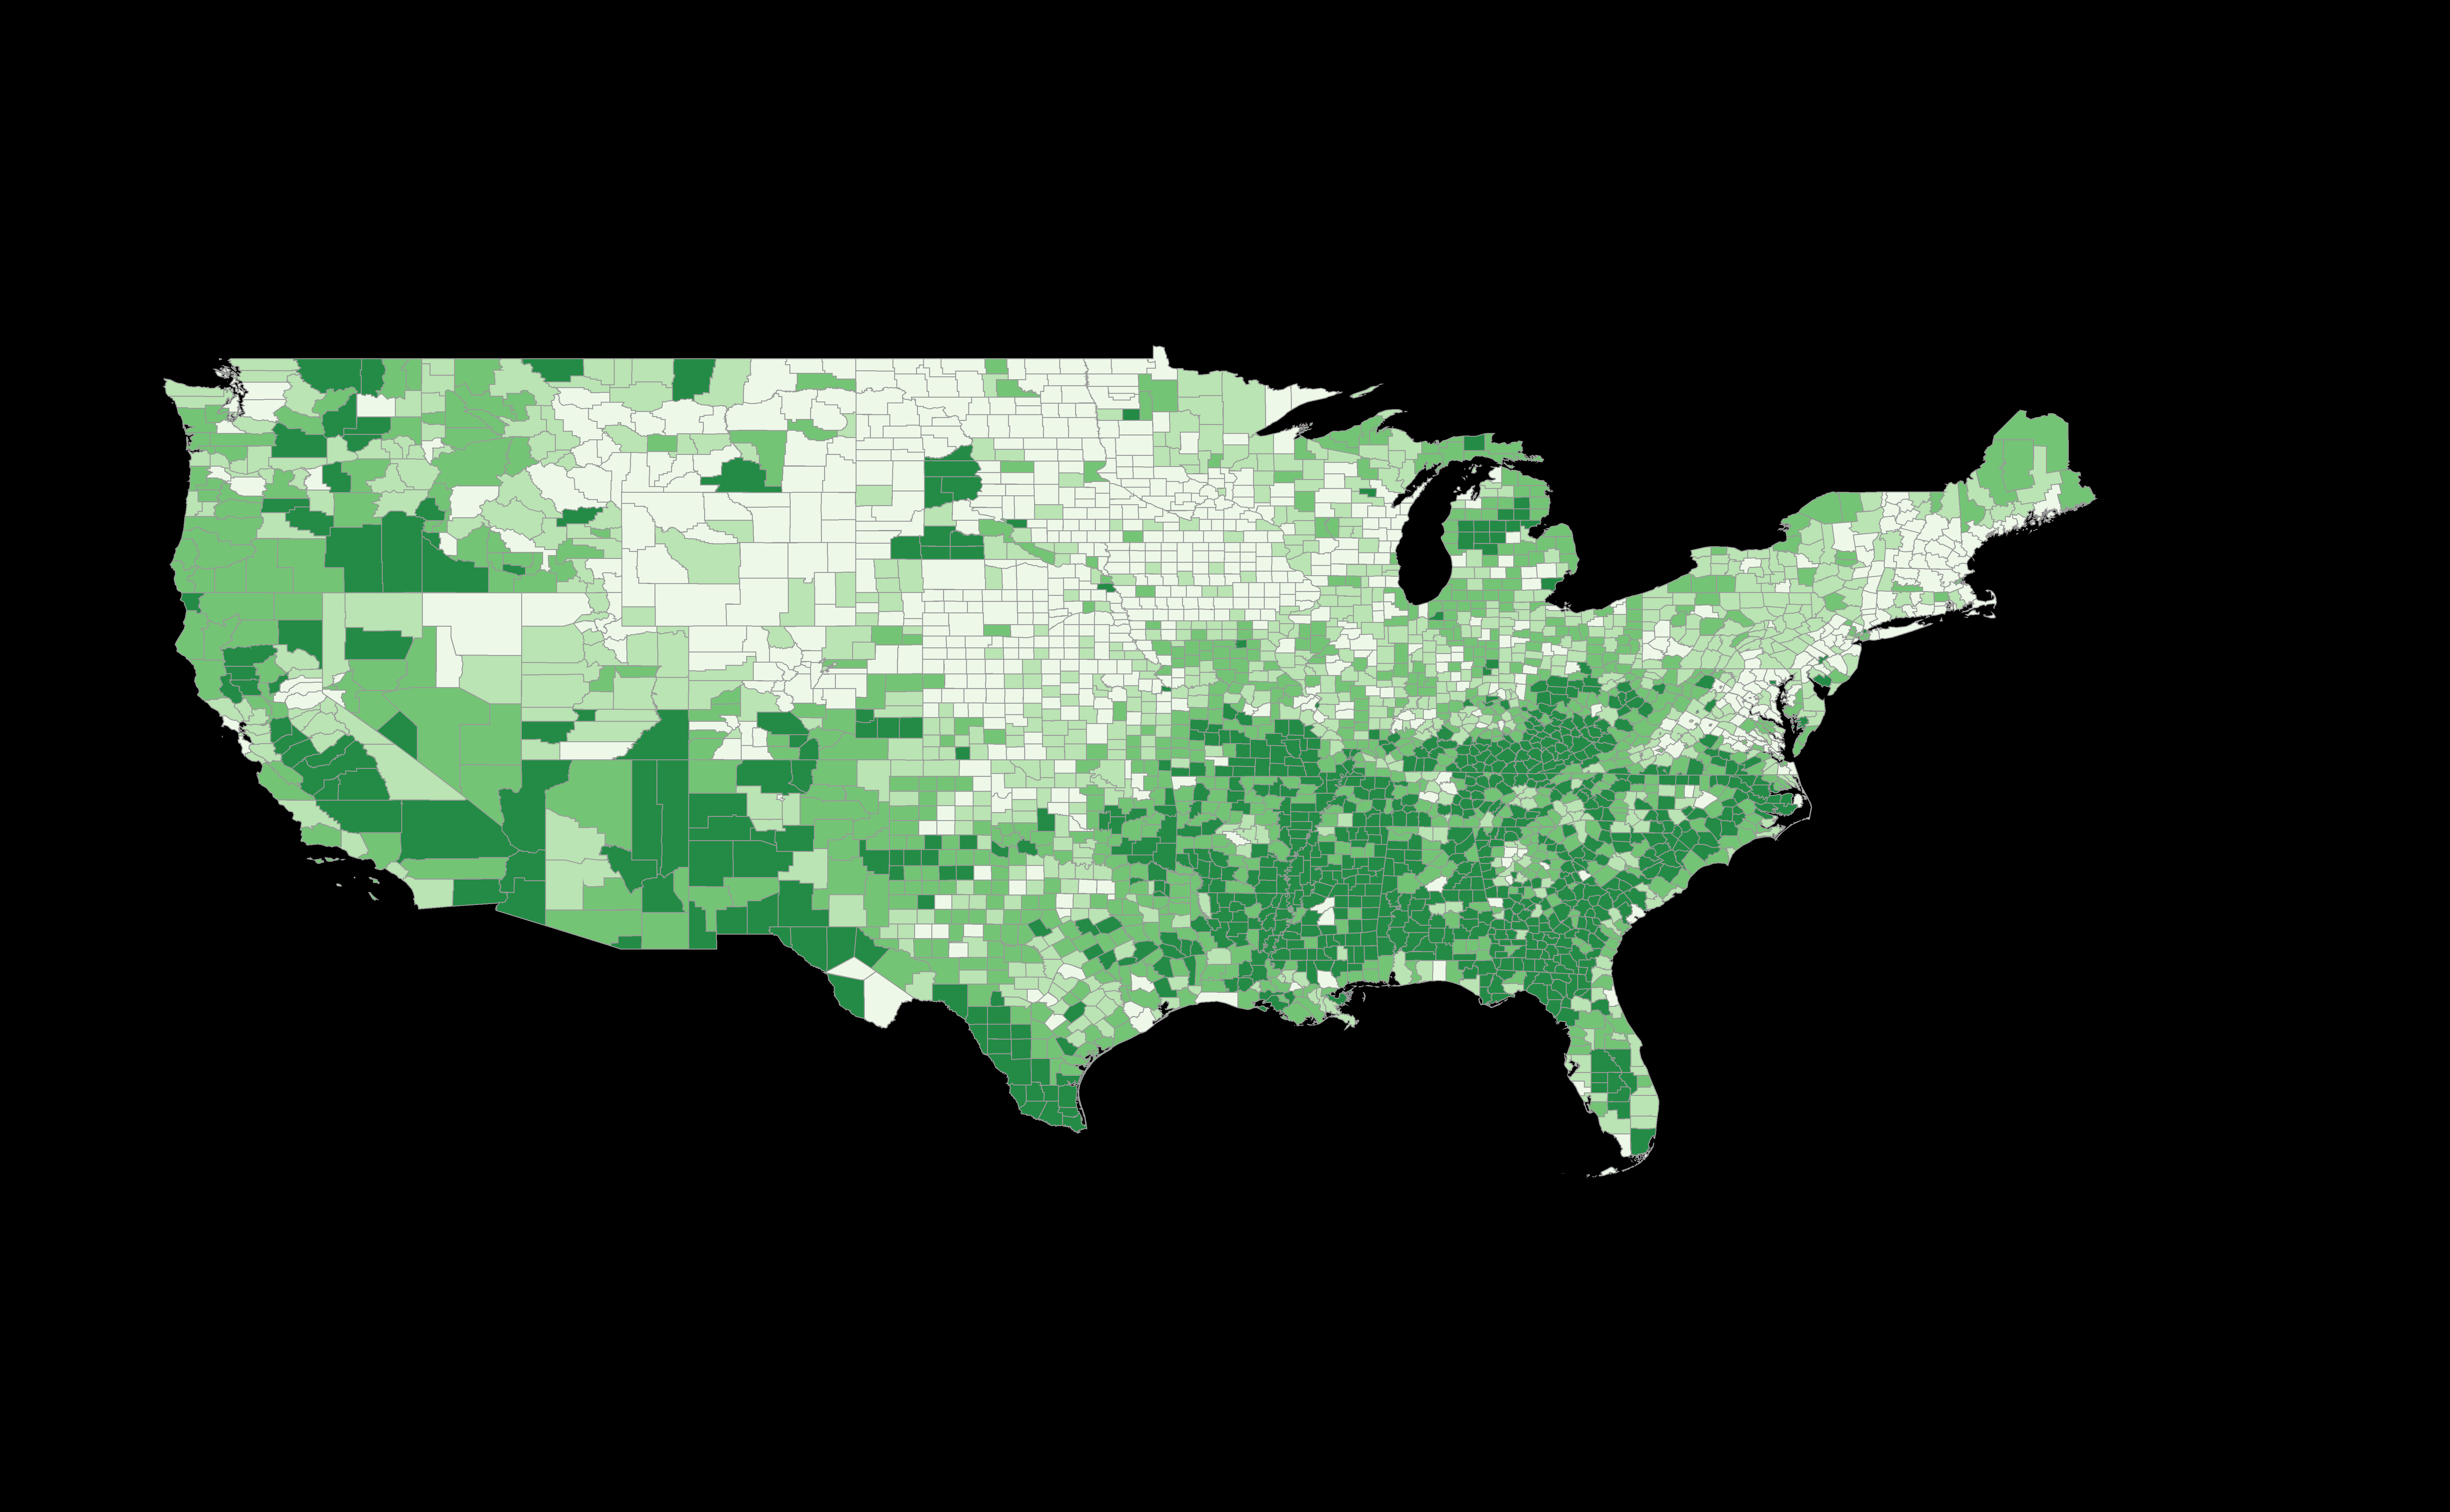
\includegraphics[width=0.8\textwidth]{figures/chloro_socioeconomic.PNG}
\captionof{figure}{Chloropeth map of Socioeconomic Status (2012-2014)}
\label{fig:chlorosocio}
\end{center}

\begin{center}
\centering
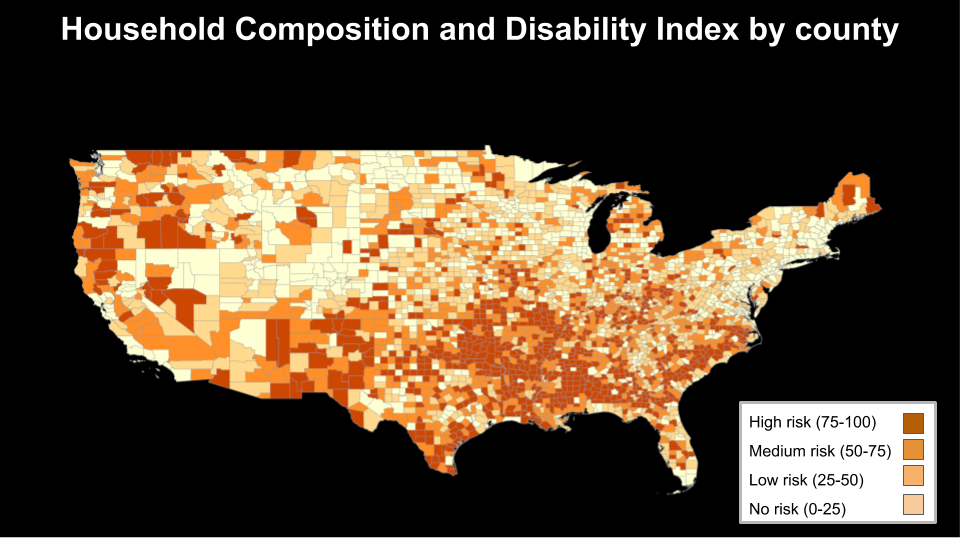
\includegraphics[width=0.8\textwidth]{figures/chloro_household_composition.PNG}
\captionof{figure}{Chloropeth map of Household Composition and Disability (2012-2014)}
\label{fig:chlorocomp}
\end{center}

\begin{center}
\centering
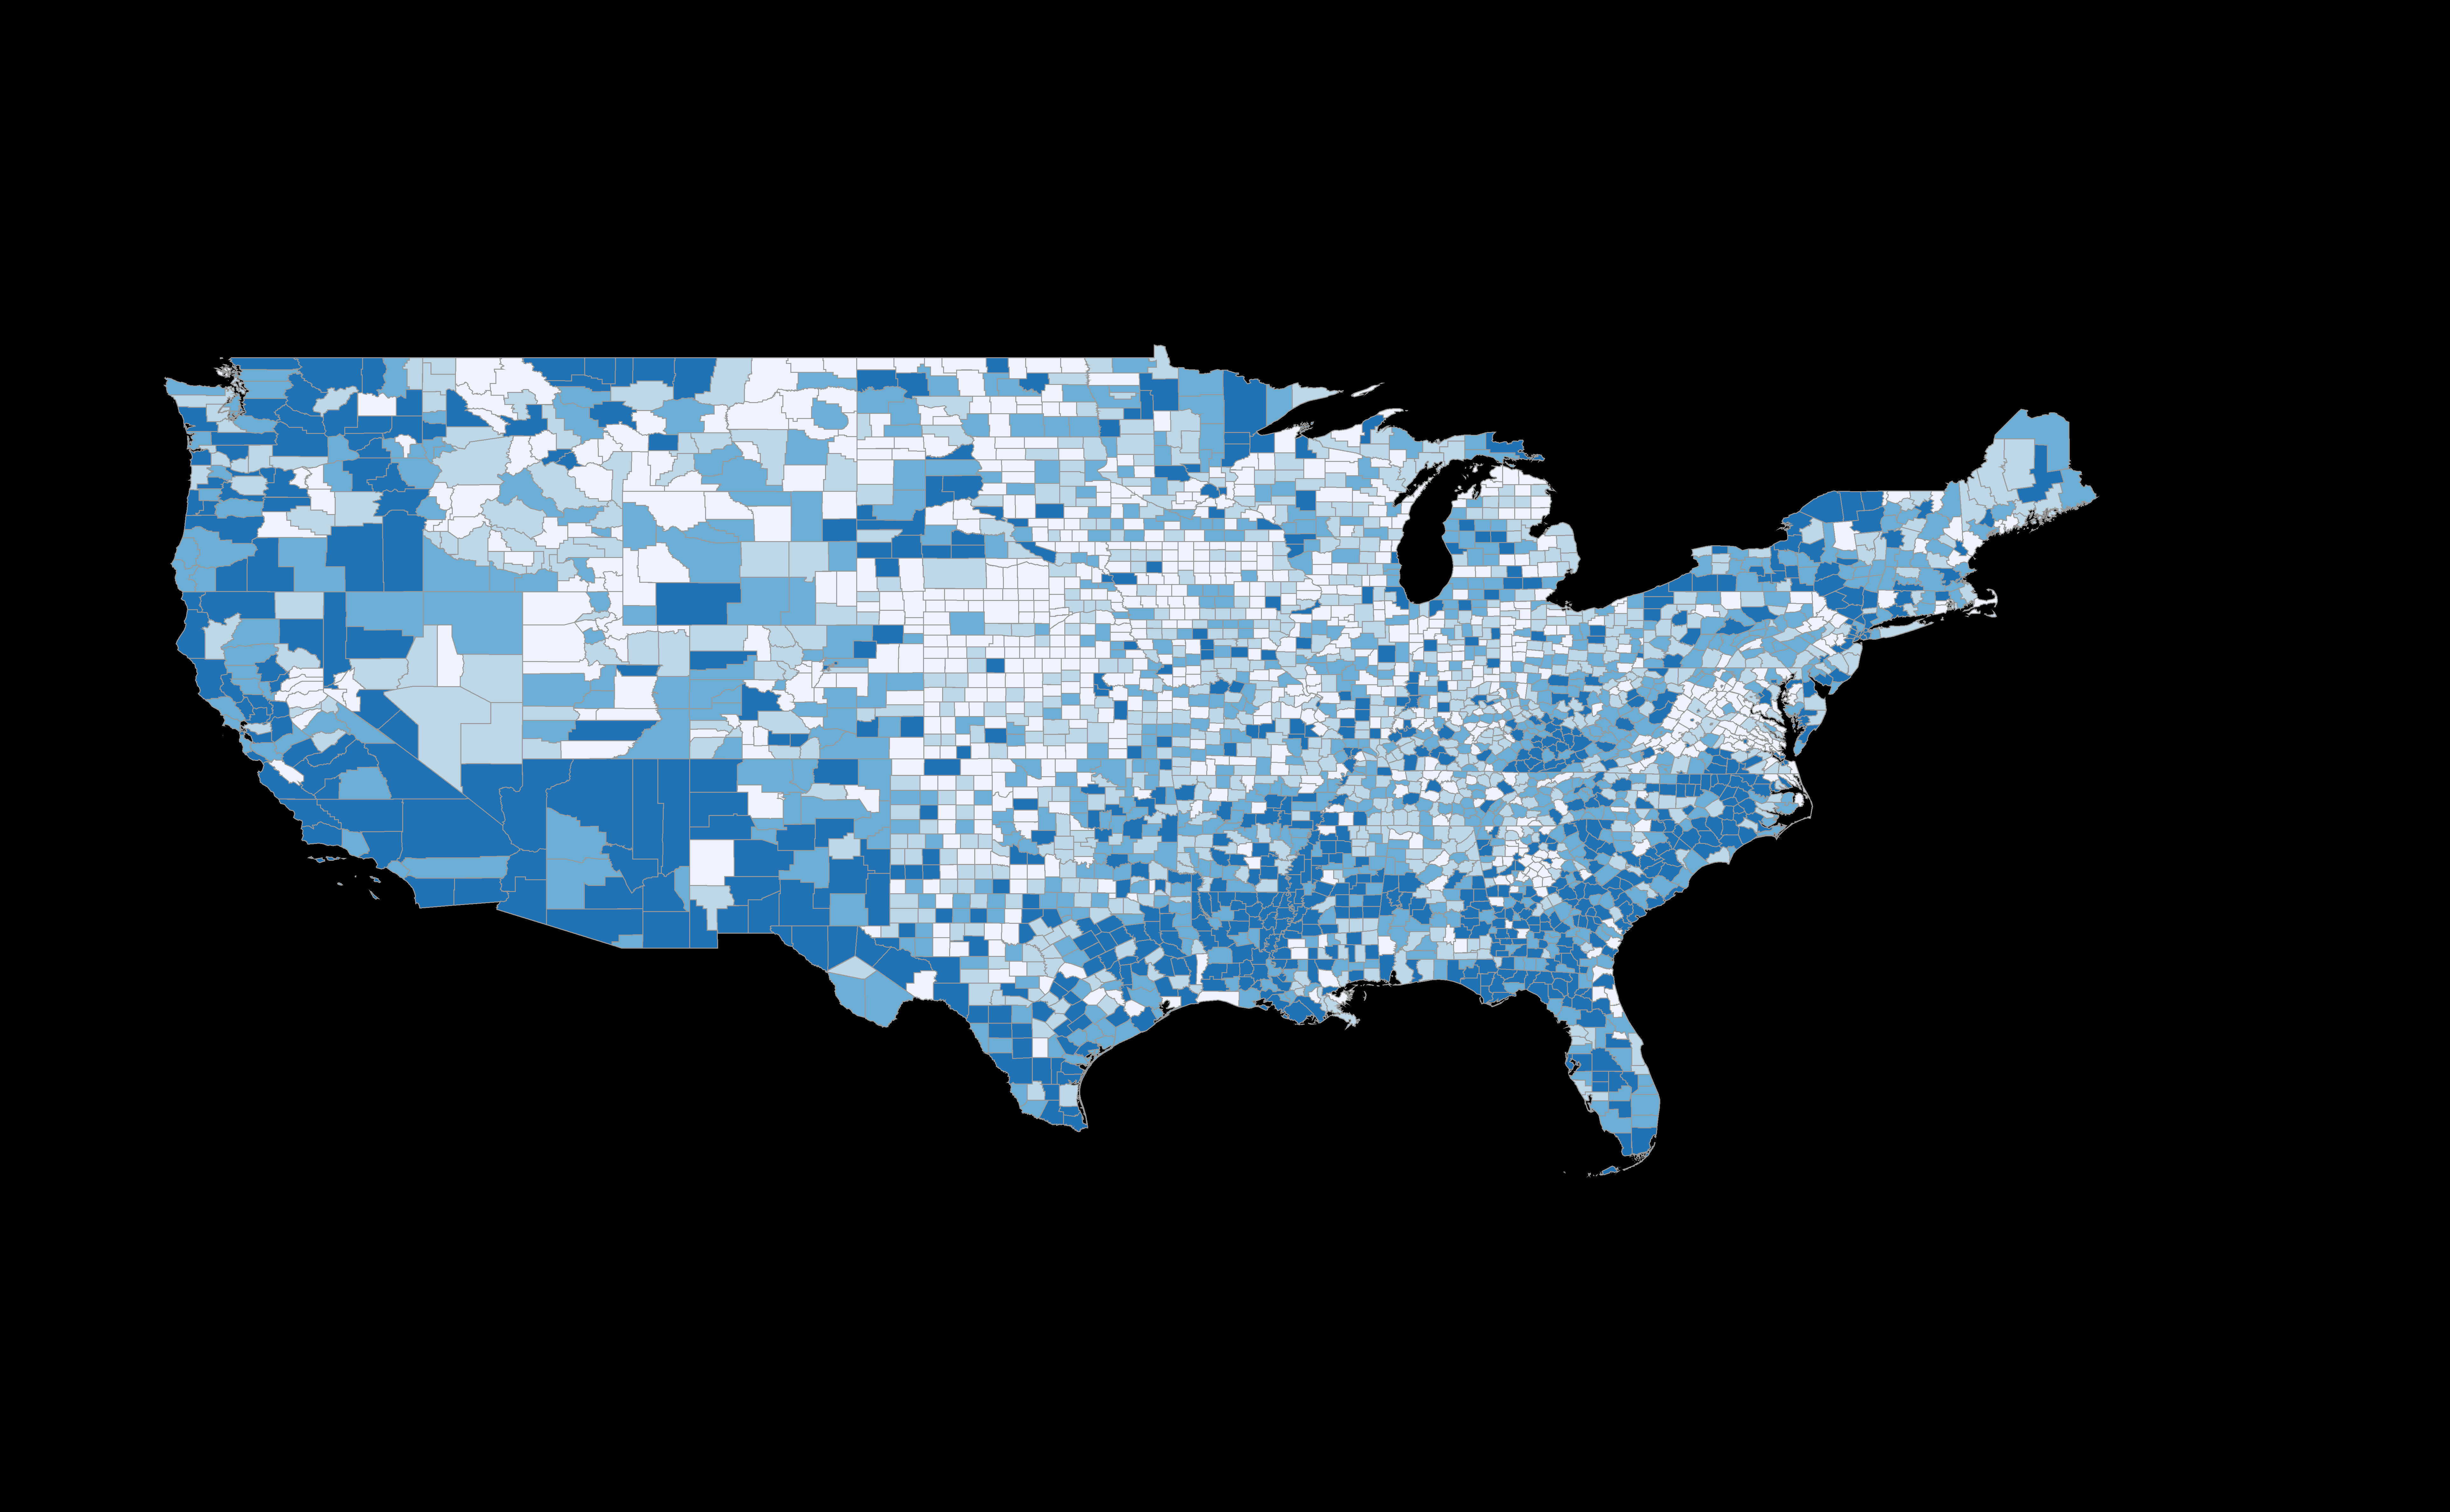
\includegraphics[width=0.8\textwidth]{figures/chloro_transportation.PNG}
\captionof{figure}{Chloropeth map of Housing and Transportation (2012-2014)}
\label{fig:chlorotrans}
\end{center}

From the Chloropeth maps we can conclude the following:
\begin{itemize}
\item Social vulnerability is a good indicator of Heart disease mortalities.
\item Both these datasets are indicative of genuine problems as they are specially smoother and not affected by population size.
\item There are some regions where there are few mortalities, but high SVI, Socioeconomic vulnerability, poor housing and transportation, and a high population which is disabled or unemployed. Certain counties in New Mexico, Arizona, Nevada, California, Oregon, and Washington score high on the SVI and all of it's subcategories but have relatively low rates of heart disease related mortalities.
\end{itemize}

\begin{center}
\centering
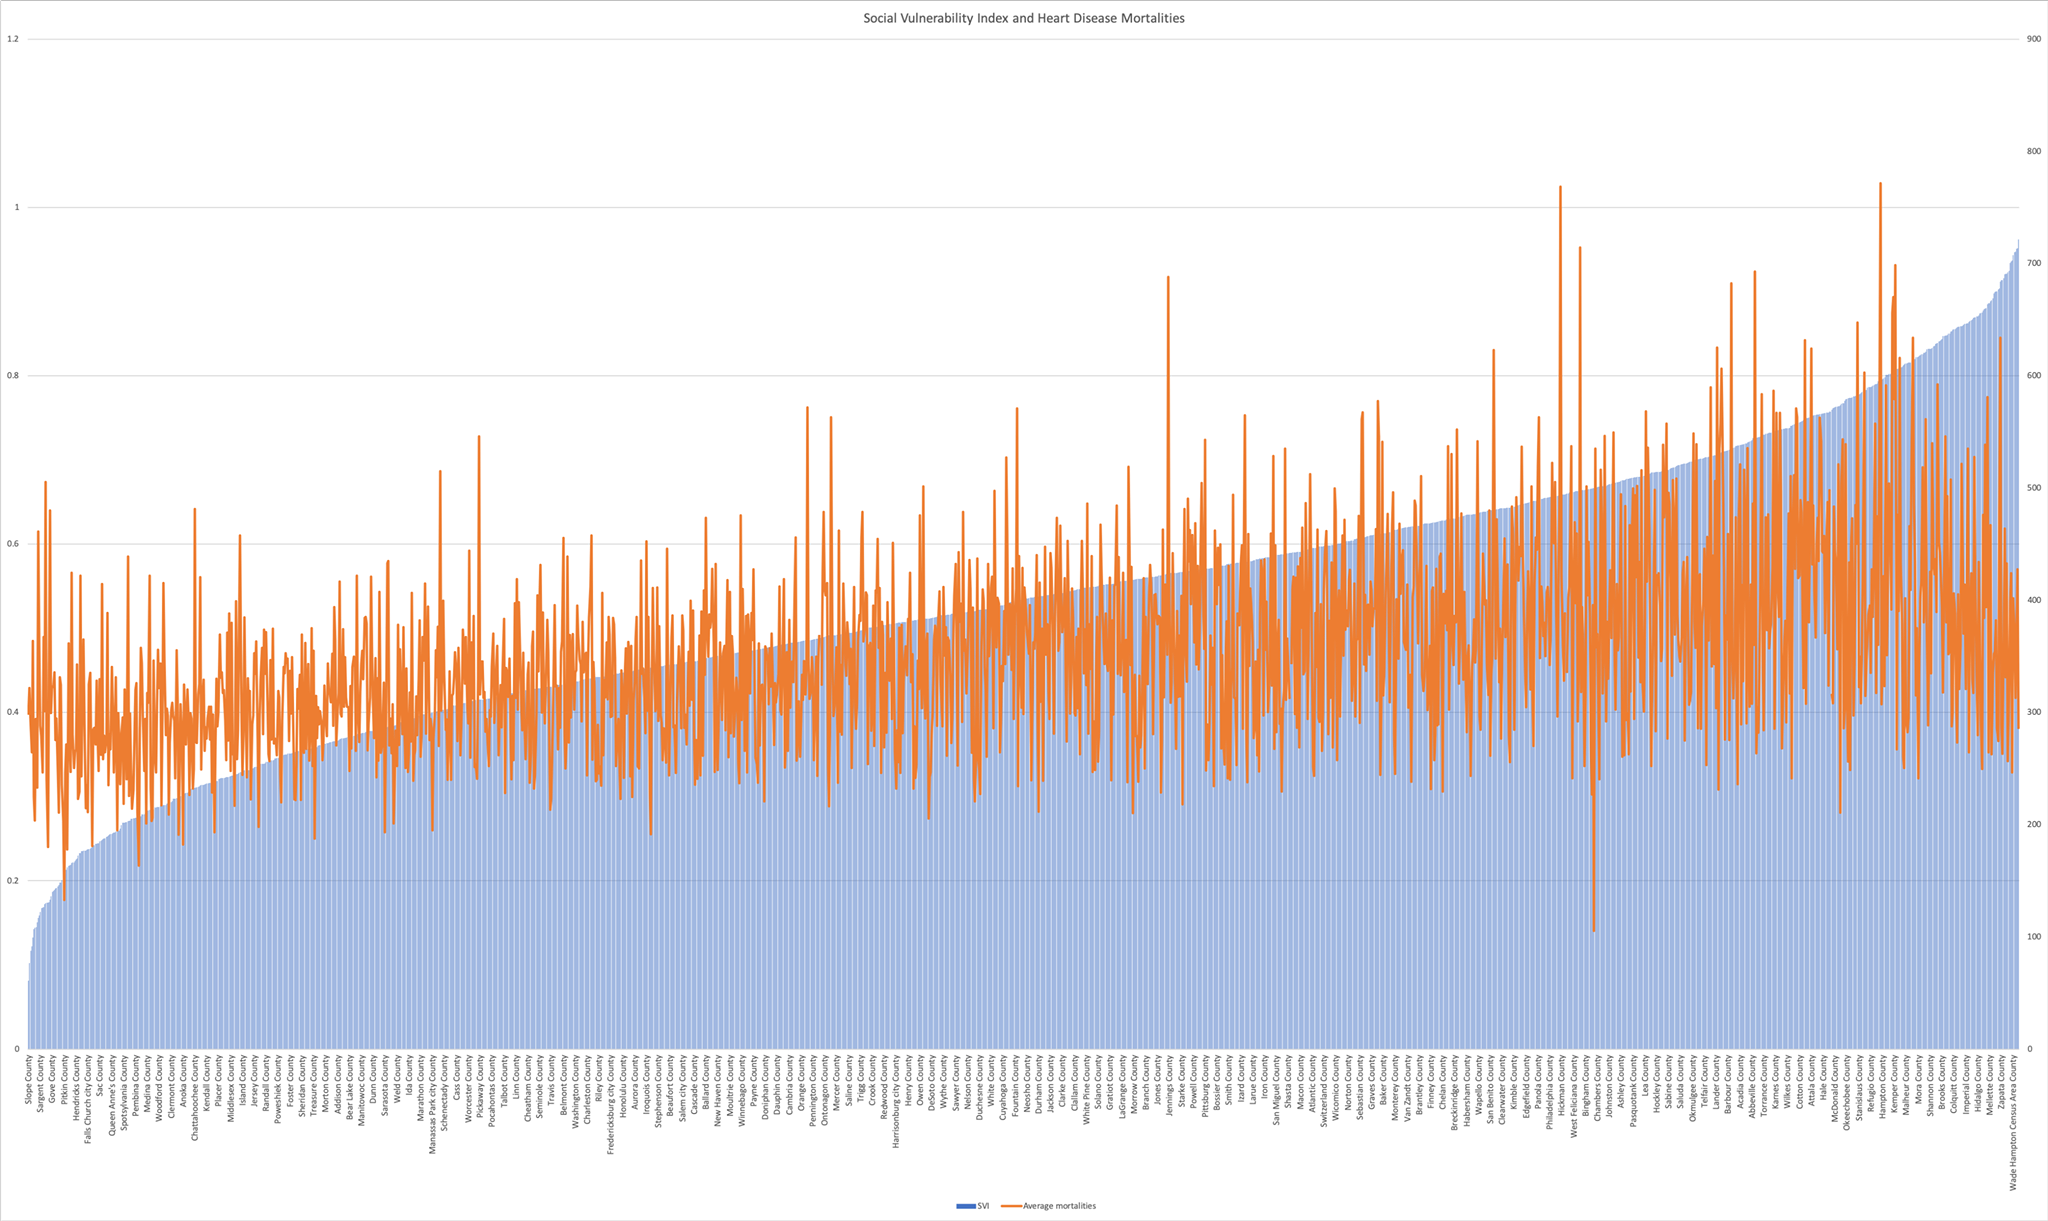
\includegraphics[width=0.8\textwidth]{figures/svi_column.PNG}
\captionof{figure}{Social Vulnerability and Heart Disease Mortality}
\label{fig:svi_column}
\end{center}

Some conclusions we can draw from Fig.~\ref{fig:svi_column}:
\begin{itemize}
\item It seems that regardless of SVI score heart disease stays pretty regular throughout the counties.
\item The only trend is that counties with higher SVI values tend to have higher highs and slightly above average heart related mortalities.
\item Surprisingly, it seems that the top 1\% of counties with the highest SVI score seem to have relatively lower heart disease related deaths.
\end{itemize}

\subsubsection{Results from Training a Machine Learning Model and Testing it on the Data}
In order to determine which model to use, we first analyzed the correlation between various metrics in the social determinants data generating the heatmap given in Fig \ref{fig:sviheatmap}.


\begin{figure}[H]
  \centering
  \begin{subfigure}{.5\textwidth}
  \centering
  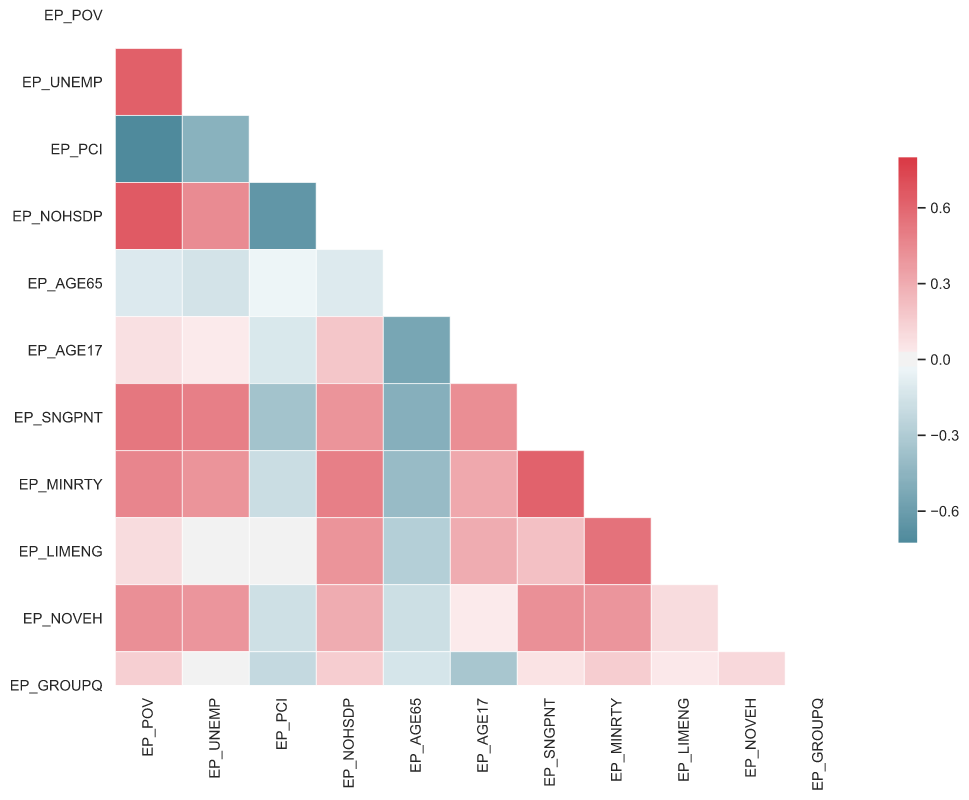
\includegraphics[width=\linewidth]{figures/ml1.PNG}
  \caption{Correlation between various social determinants}
  \label{fig:sviheatmap}
\end{subfigure}%
\begin{subfigure}{.5\textwidth}
  \centering
  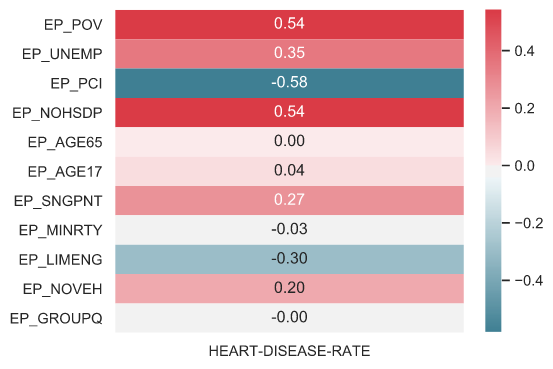
\includegraphics[width=\linewidth]{figures/ml2.PNG}
  \caption{Correleation between heart disease mortality and social determinants}
  \label{fig:hdheatmap}
\end{subfigure}
\caption{Correlation heatmaps}
\label{}
\end{figure}


From Fig.~\ref{fig:sviheatmap}, we concluded the following:
\begin{itemize}
\item There is high correlation between EP\_UNEMP and EP\_POV, i.e., poverty and unemployment rate highly correlates. Same goes for poverty vs no-high-school-diploma.
\item High correlation between minority population (EP\_MINRTY) and limited English (EP\_LIMENG), minority population and no vehicle in household(EP\_NOVEH), minority population and single parent household (EP\_SNGPNT)
\item High correlation between single parent household and poverty, which is interesting, as this is generally reversed in developing nations.
\end{itemize}

From Fig.~\ref{fig:hdheatmap}, we concluded the following:
\begin{itemize}
\item Heart-disease-death-rate highly correlates with poverty and no-high-school-diploma-household
\item Heart-disease-death-rate inversely correlates with per-capita-income and limited-English-speaking-ability
\end{itemize}


We then train two kernels (an SVM kernel and a KNN kernel) on a portion of the data (test data).
From the SVM classifier, we can get around 67\% classification accuracy, while from the KNN classifier we get around 67\% of accuracy as well.

\subsection{Management of the Presentation/Visualization}
We had created a Github repository for storing all our project related work at the beginning of the project.
All of us used this repository to store the codes and generated images/visualizations for the analysis.
This way, everyone had access to all the materials anytime they needed.
All the datasets were also stored in this repository for easy access.
Since Github is a cloud platform, it ensured that in the event all our local machines crashed for some reason, all the project materials would still persist on the cloud and be easily accessible.

\subsection{How the Visualization/Presentation Supports the Goal of the Data Science Project}
In this project, we wanted to show the relationships between heart disease mortality rate and different social determinants like median income and social vulnerability index.
The column chart with the average lines shows clearly that there is a pattern in how heart disease mortality rate varies with  median income for counties in New York State.
The Choropleth maps that we created make it very easy to understand that there is a relationship between heart disease mortality rate and the different factors.
Since column charts and Choropleth maps can be easily understood by people with no technical background, they make it easier to present the results of the analysis is a coherent manner to people from all backgrounds.
On the other hand, the confusion matrix for the SVM classifier (Fig. \ref{fig:svm}), even though it would be an important source of information for an experienced data scientist, would make little sense to someone not trained in the various data analytic methods.
\begin{figure}[H]
\centering
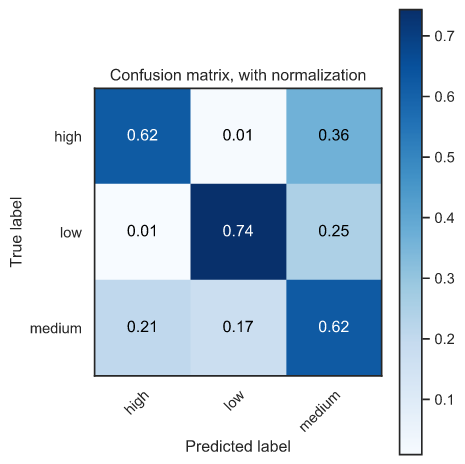
\includegraphics[width=0.4\textwidth]{figures/ml3.PNG}
\caption{Confusion matrix for the SVM classifier.}
\label{fig:svm}
\end{figure}
From this exercise, we realized that highly technical visualizations should be avoided if the goal is to make a study accessible to people from a wide range of backgrounds.
It is better to use easily understandable statistical methods like columns charts and Choropleth maps to convey data in a meaningful manner to a wide range of people.


\section{Overall Data Management Plan}
In this section, we describe our data management plan for the project.
Tha plan includes the following:
\begin{enumerate}
\item \textbf{Interoperability support}


We have put all the data used for the purpose of this project and analysis related codes and image sin a Github repository which can be accessed by the public.
The datasets are all saved as csv files and, therefore, can be easily manipulated by data manipulation software like MS Excel.

\item \textbf{Security support}


In the Github repository, have included a copy of this report.
In Section I of this report, detailed information about the source of data, metadata conventions, and provenance information has been given in detail.
Therefore, any potential user of the data can easily understand how they can validate the authenticity of the data by visiting the original source of the datasets.
Since the Github repository will be open to the public, it can be accessed without restriction, but not modified without authorization.

\item \textbf{Data ownership}


The data has been collected from public federal websites like data.gov and cdc.gov. 
Therefore, the actual owners of the data re the respective federal agents who had originally published them.
However, the other project materials that will be put in the Github repository will be owned by Rensselaer Polytechnic Institute.
Users will be able to access and use the resources, but will not be able to have ownership rights to the data.


\item \textbf{Creation of logical collections}

The datasets are separated into logical collections.
There is a separate csv file for each dataset.
The other resources that we used for the analysis of the data have also been stored in logically separate directories, making them easier to find and access.


\item \textbf{Physical data handling}


We have included back-up copies of the datasets in our public Github repository.
The original datasets can be found on data.gov and cdc.gov.
We also have a private repository that we had created for this project where we have back-ups of the datasets and all other materials associated with this project.

\item \textbf{Metadata collection, management and access}


The metadata is stored in the csv files as the header of each column.
Each column header has a name which makes it clear what the data of that column represents.
Apart from that, the data.gov and cdc.gov websites have detailed descriptions about the data.
We have included the unique identifiers of the datasets in our report, which will make it easy for people to access the original sources and read the detailed information there.


\item \textbf{Persistence}

The datasets stored in the Github repository will still persist after the course is over.
The Github repositories are permanent (until they are deleted by authorized personnel) and ca be accessed publicly.
All the project materials will also be persistent as they will be similarly stored in the Github repository.


\item \textbf{Knowledge and information discovery}


The datasets have useful metadata inside them in the form of column headers.
This allows any user to understand the relationships between the different columns. 
Moreover, in the report, we have included interesting results that conclude that there is a relationship between the data in the different datasets.
We have represented these relationships using easy to understand visualizations.
This will give all users some preliminary knowledge about the datasets if they plan to use the datasets for some kind of analysis.

\item \textbf{Data distribution and publication}

Since the Github repository will be public, users will be able to see when new changes have been made to the repository.
Github has a very elaborate system in place that allows users to see detailed information about the changes that are made to a repository.
Therefore, this system will make interested parties aware of the changes and additions to the project archive.

\end{enumerate}


\section{Conclusion}
In this project, we have tried to study the factors which affect the heart disease mortality rate of different counties across the United States.
Our results show some significant relationships between social determinant factors and heart disease mortality rates.
Hopefully, this report will be able to coherently express these relationships to the concerned authorities so that they can use this a s a basis for further investigations in this field.
Since heart disease is one of the primary killers of the US population, such investigations may help increase the average lifespan of people across the country.

\newpage
\section*{Appendix I}
\begin{itemize}
\item \emph{\textbf{data\_clean.py}} is given below:
\lstinputlisting[language=Python]{code/data_clean.py}

\item \emph{\textbf{data\_fix.py}} is given below:
\lstinputlisting[language=Python]{code/data_fix.py}
  
\end{itemize}

\section*{Appendix II}
The code used for the machine learning part of the analysis is given below:
\lstinputlisting[language=Python]{code/ml.py}

\end{document}